
\documentclass[12pt,3p]{report}
\usepackage[left=2cm, right=2cm, top=4cm]{geometry} 

\makeatletter
\def\ps@pprintTitle{%
 \let\@oddhead\@empty
 \let\@evenhead\@empty
 \def\@oddfoot{\centerline{\thepage}}%
 \let\@evenfoot\@oddfoot}
\makeatother

\newcommand{\tabitem}{~~\llap{\textbullet}~~}

\usepackage{multicol,lipsum}
\usepackage{amssymb}
\usepackage{makecell}
\usepackage{graphicx}
\usepackage{amsmath}
\usepackage{fancyhdr}
\graphicspath{ {./} }


\begin{document}


\pagestyle{fancy}
\lhead{}
\rhead{Group 15, MCEN30019 Assignment 2}

\title{
	\huge Component Selection and Evaluation\\
	\small Prosthetic Hand Development for Landmine Victims \\
	\vspace{0.5cm}
	\vspace{1cm}
	\large Group 15
}

\author{
	George Juliff\\
	\texttt{624946}
	\and
	Thomas Miles\\
	\texttt{626263}
	\and
	Adam Kues\\
	\texttt{833407}
	\and
	Lucas Brouwer\\
	\texttt{1005958}
}


\pagenumbering{gobble}
\maketitle
\vspace{2cm}

\begin{abstract}
This report describes the methodology used during the pre-prototyping phase for the mechanical design of a low cost robotic prosthetic hand. Several feasible subsystem designs are proposed and their suitability in combination is determined using a set of objective evaluation functions. Due to the systematic nature of this early design process, the system's initial concept design is shown to be well optimised to best achieve our design targets while accounting for limitations in cost and manufacturing capability specific to the product.
\end{abstract}

\pagebreak

\tableofcontents

\pagebreak

\pagenumbering{arabic}

\part{Forward}
\section{Summary of Design Criteria}
	\subsection{Essential}	\label{ess}
	
		\begin{center}
	\begin{tabular}{ |c|c|c| } 
 \hline
 Criterion & Objectives & Evaluation Function \\ 
 \hline\hline
 $E_1$ & $Obj3$ & \makecell[l]{Met if: \\
 \tabitem Portion attached to forearm weighs less than 500g. \\
 \tabitem Unit does not cause pain, irritation or significant discomfort. \\
 \tabitem Forearm size does not exceed 1.1 times natural forearm width.} \\
 \hline
 $E_2$ & $Obj_2$ & \makecell[l]{Met if: \\
 \tabitem Unit costs less than \$500AU to manufacture. \\
 \tabitem Unit takes less than 2 weeks to manufacture.} \\ 
 \hline
 $E_3$ & $Obj_{1,3}$ & \makecell[l]{Met if: \\
 \tabitem Unit palmer pinch force is greater than 65N. \\
 \tabitem Unit closes at 115$^{\circ}$/s. \\
 \tabitem Unit has a idle battery life of 10 hours. \\
 \tabitem Software has gesture classification accuracy above 90\%.} \\
 \hline
 $E_4$ & $Obj_{2,3}$ & \makecell[l]{Met if: \\
 \tabitem Unit IP 54 rated on exposed sections. \\
 \tabitem Unit components have an expected 1 year lifespan.} \\ 
 \hline
		\end{tabular}
	\end{center}

	\subsection{Desirable} \label{des}
		\begin{center}
			\begin{tabular}{ |c|c|c|c| } 
 \hline
 Criterion & Objectives & Evaluation Function & Definitions \\ 
 \hline\hline
 $D_1$ & $Obj_1$ & $\text{min} \left \{\dfrac{M_{RF}}{M_{RF_{max}}},1 \right \}$ &  \makecell[l]{
  \vspace{1mm}
 $M_{RF}$: Impact strength (N impulsive) \\
 $M_{RF_{max}}$: 140N
 \vspace{1mm}
 } \\
 \hline
 
 $D_2$ & $Obj_3$ & $\text{max} \left \{1-\dfrac{M_L}{M_{L_{max}}}, 0 \right \}$ &  \makecell[l]{
 \vspace{2mm}
 $M_L$: Noise in actuation (dB) \\
 $M_{L_{max}}$: 50dB
 } \\
 \hline

 $D_3$ & $Obj_1$ & $D_3 =  \cfrac{\sum_{n=1}^{n=\text{DOF}} \left(k_n \cdot \text{min}\{\frac{M_{RS}}{M_{RS_{max}}},1\} \right)}{\text{DOF}}$ &  \makecell[l]{
 $M_{RS_n}$: Rotation speed (degree n, $^\circ$/s). \\
 $M_{RS_{max}}$: $230^\circ$/s
 } \\
 \hline
 $D_4$ & $Obj_3$ & $D_4 = \cfrac{p_{range}}{100} \times d  \times I $ &  \makecell[l]{
 **variable definitions***
 } \\
 
 \hline
		\end{tabular}
	\end{center}



\pagebreak

\part{Mechanical Design}
\begin{multicols}{2}

	\section{Fingers}
TODO explain general material selection reasoning (in that they are all printed n' shit)
	
	
		\subsection{Transmission}
		
		
			\begin{enumerate}
			\item \textbf{Flexor tendon through sheaths} {

%TODO figures are fukd
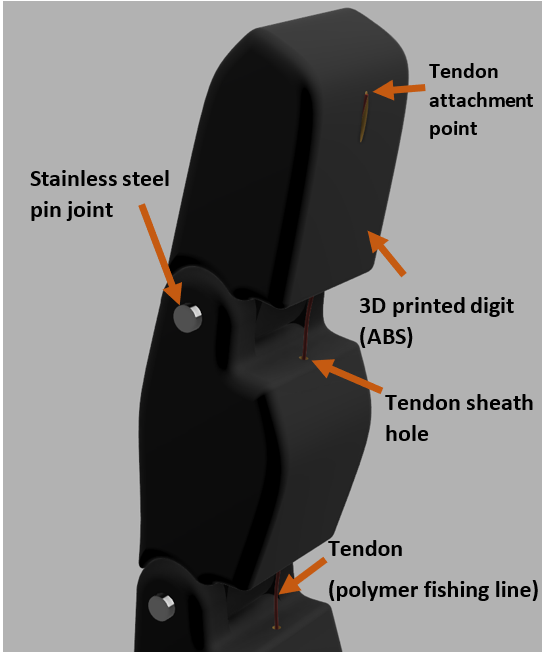
\includegraphics[scale=0.5]{tendon.PNG}
			
				This method of articulating the finger relies on closely mimicking a real finger and using a tendon to provide one degree of freedom to each finger and the thumb. These tendons will be controlled by motors either in the hand or wrist. Multiple fingers can be attached to a single motor, reducing degrees of freedom, but potentially improving other characteristics such as weight.
				
			}
			\item \textbf{Felxor tendon using pulleys} {
							
				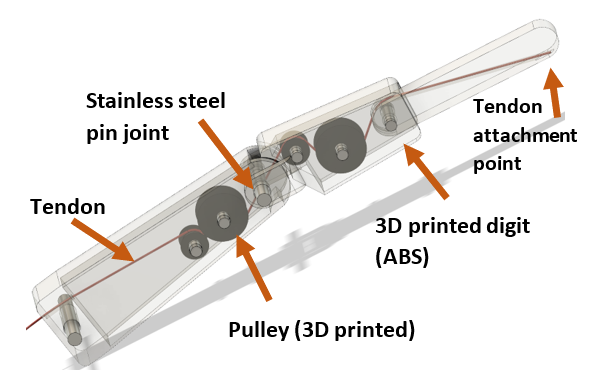
\includegraphics[scale=0.5]{pulley.PNG}
				A more novel tendon design based on xxCITATIONxx, which provides a slight mechanical advantage over design 1, and has a smoother closing action since pulley placement distributes load between finger digits more evenly. 
			}
			\item \textbf{Geared metacarpo-phalangeal joint} {
			
				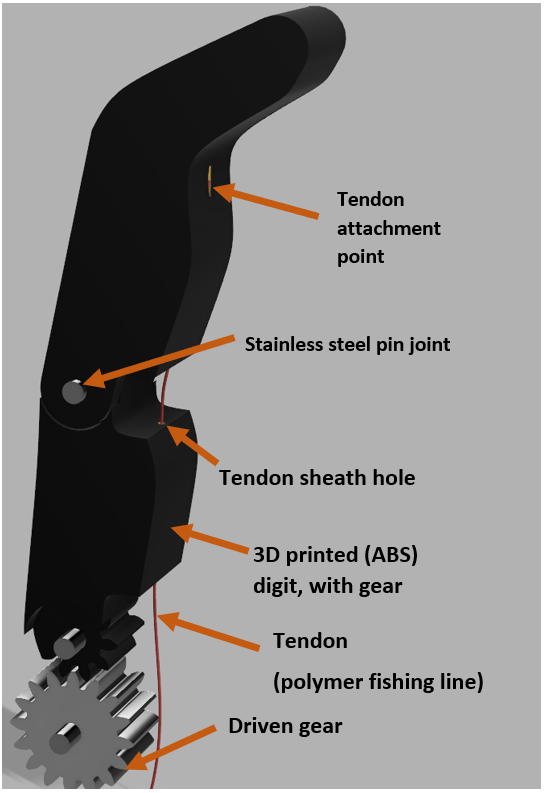
\includegraphics[scale=0.5]{gear.PNG}
				This method of articulating the finger ensures the finger closes evenly, using a tendon for the upper joint, attached to the same motor that drives the gear that closes the lower joint, prevents one joint closing at a different rate to the others. Furthermore, transmission of power to the finger via a gear will allow for actuation in both directions, and is less prone to failure than fishing line, which may snap under extreme loads.
			}		
			\end{enumerate}
			
		\subsection{Joints}
		
		\begin{enumerate}
		\item \textbf{Pin joint} {
		
		As pictured above TODO
		}
		\item \textbf{Elastic joint} {
		
		xxCITATIONxx type
		}
		\item \textbf{Silicone} {
		
		fully rubber TODO
		}
		\end{enumerate}

	


\subsection{Degrees of freedom and constraints}
		
		In order to satisfy essential criteria $E_3$, the hand must be able to, at minimum, open and close with a force of 65 newtons. This can be achieved using a single degree of freedom (DOF), closing all fingers simultaneously. Each finger transmission design explored have a single degree of freedom for this reason. 
		
		The total number of constraints and DOF's for a finger depends on the joint morphology.



	\section{Thumb}
	
		\subsection{Degrees of freedom and constraints}

		
		\subsection{Transmission of opposable joint}
			\begin{enumerate}
			\item \textbf{Rigid} {
			
			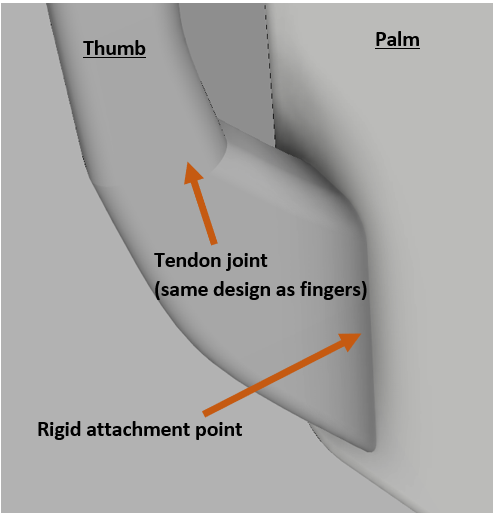
\includegraphics[scale=0.55]{rigid_thumb.PNG}
						This design allows for the lower thumb joint and the palm to be 3D printed as part of the same piece, reducing assembly difficulty.
			}

			\item \textbf{Manual operation} {
				
				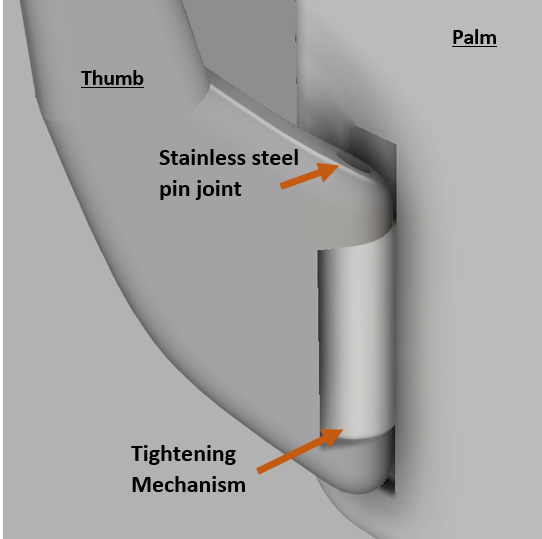
\includegraphics[scale=0.45]{man_thumb.PNG}
				This joint is manually articulated using the operator's other hand, allowing different thumb orientations to tackle a wider range of tasks. For this to be useful however, the joint needs to be stiff enough to remain in a set position during use. This can be achieved either using a very snug fit on the pin joint, have a thread on the pin joint by which the user can tighten a nut to lock it in place, or using a spring-ratchet system similar to that in figure: TODO
			}
			\item \textbf{Geared} {
				
				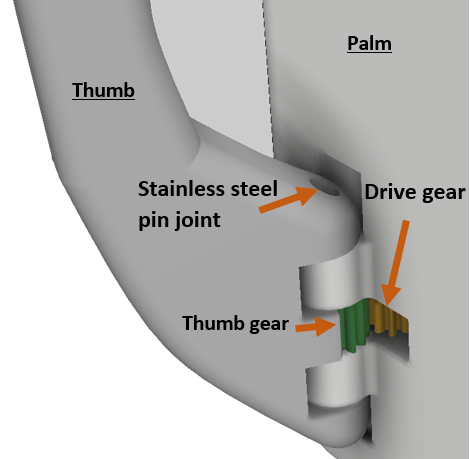
\includegraphics[scale=0.5]{Driven_thumb.PNG}
				This method is analogous to the geared joint finger design, however it allows one more degree of freedom since the second joint can be operated independently of opposable rotation. 
			}		
			\end{enumerate}	
		
		
		
	\section{Wrist}
	
		\subsection{Degrees of freedom and constraints}
		TODO briefly explain (with cite) why this is needed and why only 1 DOF is reasonable
		
		\subsection{Transmission}	
		
			
			\begin{enumerate}
			\item \textbf{Rigid} {
			
				A fixed wrist joint is the simplest to manufacture, and will reduce the overall weight due to the need for one fewer motors.
			}	
			\item \textbf{Planetary gearbox} {

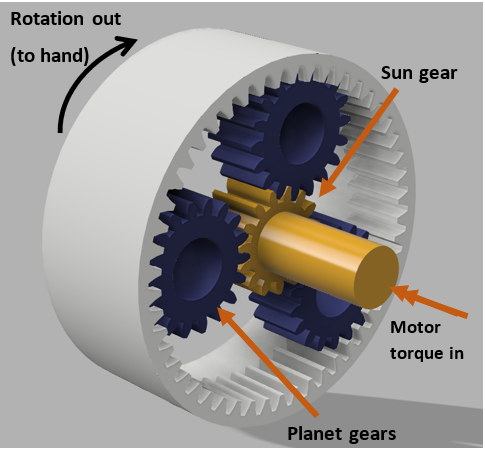
\includegraphics[scale=0.6]{planet.PNG}
The planetary gearbox design does not require a bearing since the outer ring can be embedded into the hand side of the prosthetic, while planet gears can be made captive using a herringbone tooth pattern. It also allows for a very high gear ratio without the need for multiple step-downs, since 3D printing gives us the ability to manufacture any sized gears required. Due to the number of gears, inaccuracy in 3D printed teeth, and rate of rotation of the sun gear, a planetary system will be a fair amount louder than alternate methods during operation.
			}	
			\item \textbf{Belt Drive} {

Belt drives can mitigate the noise factor associated with printed plastic on plastic gears, however achieving high gear ratios may require more than one belt for the same ratio a planetary gearbox could achieve. Furthermore, physical space within the arm may be a concern, since the rotation required is in the axis of the arm, the belt and pulley are limited in size.
			}	
			\end{enumerate}


	
	
	\section{Socket}
		
		\subsection{Solid, generic}
		

		
		\subsection{Solid, 3D printed}
		
		
		
		\subsection{Non-rigid/Strap on}
		
				\pagebreak
			\end{multicols}	
	\section{Evaluation}
\begin{tabular}{|c|c|c|c|c|c|c|c|c||c|}
\hline 
 & $E_1$ & $E_2$ & $E_3$ & $E_4$ & $D_1$ & $D_2$ & $D_3$ & $D_4$ & $D_{overall}$ \\ 
\hline 
Finger 1. & • & • & • & • & • & • & • & • & •\\ 
\hline 
Finger 2. & • & • & • & • & • & • & • & • & •\\ 
\hline 
Finger 3. & • & • & • & • & • & • & • & • & •\\ 
\hline 
Joint 1. & • & • & • & • & • & • & • & • & •\\ 
\hline 
Joint 2. & • & • & • & • & • & • & • & • & •\\ 
\hline 
Joint 3. & • & • & • & • & • & • & • & • & •\\ 
\hline 
Thumb 1. & • & • & • & • & • & • & • & • & •\\ 
\hline 
Thumb 2. & • & • & • & • & • & • & • & • & •\\ 
\hline 
Thumb 3. & • & • & • & • & • & • & • & • & •\\ 
\hline 
Wrist 1. & • & • & • & • & • & • & • & • & •\\ 
\hline 
Wrist 2. & • & • & • & • & • & • & • & • & •\\ 
\hline 
Wrist 3. & • & • & • & • & • & • & • & • & •\\ 
\hline 
Socket 1. & • & • & • & • & • & • & • & • & •\\ 
\hline 
Socket 2. & • & • & • & • & • & • & • & • & •\\ 
\hline 
Socket 3 & • & • & • & • & • & • & • & • & •\\
\hline
\hline 
 & $E_1$ & $E_2$ & $E_3$ & $E_4$ & $D_1$ & $D_2$ & $D_3$ & $D_4$ & $D_{overall}$ \\
\hline 
Full 1 & • & • & • & • & • & • & • & • & • \\ 
\hline 
Full 2 & • & • & • & • & • & • & • & • & • \\ 
\hline 
Full 3 & • & • & • & • & • & • & • & • & • \\ 
\hline 
\end{tabular} 




\pagebreak
\part{Actuator Selection}

\begin{multicols}{2}
	\section{Motors}
	
		\subsection{Motor 1}
	
	
	
		\subsection{Motor 2}
		
		
		
		\subsection{Motor 3}



	\section{Evaluation}


\newpage
\appendix



\bibliographystyle{elsarticle-num}


\bibliography{sample}
\end{multicols}


\end{document}
